\pagebreak
\section{Deferred Shading}

\begin{center}
\emph{{\small Tobias Graf}}
\end{center}

\bigskip

\subsubsection*{Einleitung} Um aus der entstandenen Drahtgitter - Oberfläche des Marching Cubes Algorithmus eine Näherung zu einer Wasseroberfläche zu erzielen wird Deferred Shading verwendet. In diesem Kapitel wird kurz erläutert was Deferred Shading generell ist und das ShaderProgramm daraus einen Transparenten Wassereffekt erreicht.

\subsection*{Deferred Shading} Ursprünglich ist Deferred Shading eine Technik der Computergrafik um die Lichtberechnung von der Geometrieberechnung zu trennen. Sie erlaubt durch das Reduzieren der Komplexität wesentlich mehr Lichtobjekte in einer Szene als bei klassischen Rendermethoden, in denen anhand der Tiefe, Normale und Farbwert eines Eckpunktes in Korrelation einer Lichtquelle die Dargestellte Farbe berechnet wurden. Beim Deferred Shading werden durch sogenannte Framebufferobjekte (FBO) Tiefenwerte, Normale und Farbe der Geometrien in eine Textur mit Bildschirmauflösung gerendert. Statt nun für jeden Geometrischen Eckpunkt den Farbwert zu berechnen wird dies nun für jeden Pixel angewandt wodurch der Aufwand von $O(m*n)$ auf $O(m+n)$ reduziert wird. Nachteilig dabei ist das zwar weniger Hardwareanforderungen benötigt werden um die gleiche Szene zu rendern, jedoch der Speicherverbrauch extrem ansteigt da die Texturen im Grafikkartenspeicher vorgehalten werden müssen.\\
Relativ schnell Entwickelten sich vielfältige Nutzungen der Technik zum einsetzen von Postprocessing Effekten, wodurch völlig neue Optimierungstechniken zur Verfügung stehen. Gängige Bildbearbeitungsfilter wie Weichzeichnen und Kantenerkennung sind einfach in einem ShaderProgramm einzusetzen und erlauben dadurch eine deutlich verbesserte Grafikqualität.
Zusätzlich erlaubt Deferred Shading das erstellen von ShadowMaps um Schatteneffekte von Objekten Darzustellen, indem einfach in einem zusätzlichen Rendering Schritt die Szene aus der Sicht der Lichtquelle gerendert wird, und diese Resultierende Textur als ShadowMap verwandt wird.

\subsection*{Unser Ansatz} Angelehnt an den das verfahren von Simon Green aus dem GDC Vortrags \cite{DSGDC} erfolgte zuerst die Implementation mehrerer Framebufferobjekte die als einzelne Rendertargets benutzt werden um verschiedene Aspekte der Szene einzeln in Texturen zu Rendern. Da bereits eine Mesh - Oberfläche gegeben ist fallen einige im Vortrag genannte Schritte betreffend die Texturerstellung der Oberflächen weg.\\
Zur Lichtberechnung wir das Phong-Modell verwendet, der Nachteil dieser relativ simplen Belichtungsberechnung für Diffuse und Spekulare Lichtanteile ist der sogenannte "Nasse" Effekt der jedoch zur Darstellung einer Wasseroberfläche schon automatisch das wesentliche mitbringt.
\newpage
Die Aufteilung erfolgt in folgende FBO und Grafiken:
\begin{itemize}
\item Hintergrund
\item Thickness
\item Partikel
	\begin{itemize}
	\item Farbwert
	\item Tiefenwert
	\item Welt - Koordinate
	\item Normale
	\item Spekulare Farbe
	\item Diffuse Farbe
	\end{itemize}
\end{itemize}  

\noindent Das getrennte Rendern des Hintergrundes ist notwendig um den Transparenz Effekt zu erreichen da dies eine schwäche von Deferred Shading ist da man keinen nutzen aus der OpenGL Blend Funktion ziehen kann wenn die einzelnen Geometrien in getrennten FBO gezeichnet werden. Die Thickness bestimmt im abschließenden Bild die Hauptsächliche Transparenz der Oberfläche. Der Partikel FBO schreibt die einzelnen Parameter mit denen die Lichtberechnung und die Farbgebung des Objektes in die jeweiligen Texturen.
\begin{center}
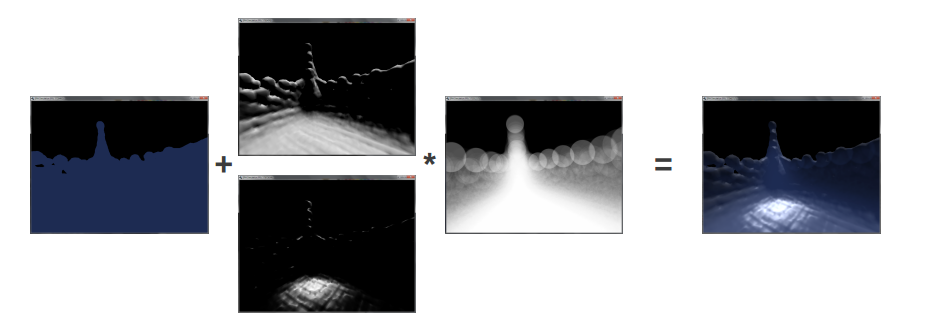
\includegraphics[scale=0.7]{images/Dereffered}
\end{center}
\noindent Das Letzte ShaderProgramm verknüpft die einzelnen Texturwerte mit unterschiedlichen Verhältnissen um eine leichte Transparenz der Oberfläche zu erhalten die durch den Thickness Parameter tritt bei einer hohen Dichte eher der Farbwert der Oberfläche hervor und die Transparenz lässt ein wenig nach.